\newcommand*{\tl}{\mathrm t}  % translation 平动
\newcommand*{\rt}{\mathrm r}  % rotation 转动
\newcommand*{\vb}{\mathrm v}  % vibration 振动

\chapter{Boltzmann统计}

\section{理想气体}
\label{sec:ideal gas}

理想气体满足非简并条件($\e\alpha\gg 1$),符合半经典Boltzmann分布。
粒子的运动可分为质心的平动(translation)、粒子内部的振动(vibration)和粒子整体的转动(rotation)三个相互独立的运动。

\subsection{平动}
\label{ssec:translation}

由\exmref{exm:monatomic molecule},单个粒子的平动能量和态密度为
\[
	\varepsilon_\tl=\frac1{2m}(p_x^2+p_y^2+p_z^2),\quad g(\varepsilon)=\frac{2\pi V}{h^3}(2m)^{3/2}\sqrt\varepsilon.
\]
在能量准连续的条件下,配分函数
\begin{equation}
	Z_\tl=\int\zti g(\varepsilon)\e{-\beta\varepsilon}\d\varepsilon=\frac{2\pi V}{h^3}\int\zti\sqrt\varepsilon\e{-\beta\varepsilon}\d\varepsilon=V\biggkh{\frac{2\pi m}{h^2\beta}}^{3/2}.
\end{equation}
考虑只有平动的情况,如单原子分子,
\footnote{统计力学部分,$n:=V/N$表示粒子数密度,而不再表示摩尔数。}
\[
	\e{\alpha}=\frac{Z_\tl}N=\frac1n\biggkh{\frac{2\pi m\kB T}{h^2}}^{3/2},
\]
说明在稀薄、高温、大质量的情况下,$\e\alpha\gg 1$,满足非简并条件。
另外,非简并条件也可以写成$\e{-\alpha}=n\lambda_T^3\ll 1$的形式,
其中$\lambda_T$是能量为$\pi\kB T$时的de Broglie波长
\begin{equation}
	\label{eq:de Broglie wavelength}
	\lambda_T=\frac{h}{\sqrt{2\pi m\kB T}}.
\end{equation}
基于配分函数,可得平动所贡献的内能、比热、压强和熵:
\footnote{经典统计采用经典Boltzmann分布推导出来的熵甚至不是广延量,应修正为半经典Boltzmann分布。}
\begin{subequations}
	\begin{align}
		U_\tl&=-N\pv{\ln Z_\tl}\beta=\frac32N\kB T,\\
		C_{V,\tl}&=\pu[V]{U_\tl}T=\frac32N\kB,\\
		p&=\frac N\beta\pv{\ln Z_\tl}V=\frac{N\kB T}V,\\
		S_\tl
		% &=N\kB\biggkh{\ln Z_\tl-\beta\pv{\ln Z_\tl}\beta-\ln N+1}\\
		&=\frac52N\kB+N\kB\ln\biggfkh{\frac VN\biggkh{\frac{2\pi m\kB T}{h^2}}^{3/2}}.
	\end{align}
\end{subequations}
将状态方程$pV=N\kB T$与实验得到的理想气体状态方程\eqref{eq:pV=nRT}对比,可得理想气体常数$R=\kB\NA$。
由于国际单位制直接指定了$\kB$和$\NA$的值,因此$R$的数值也是精确的。

\begin{theorem}
	{Maxwell速度分布律}{Maxwell distribution of velocities}
	速率在$(v,v+\d v)$范围内的粒子数密度为
	\begin{equation}
		f(v)\d v=4\pi n\biggkh{\frac m{2\pi\kB T}}^{3/2}\e{-mv^2/2\kB T}v^2\d v.
	\end{equation}
	\begin{center}
		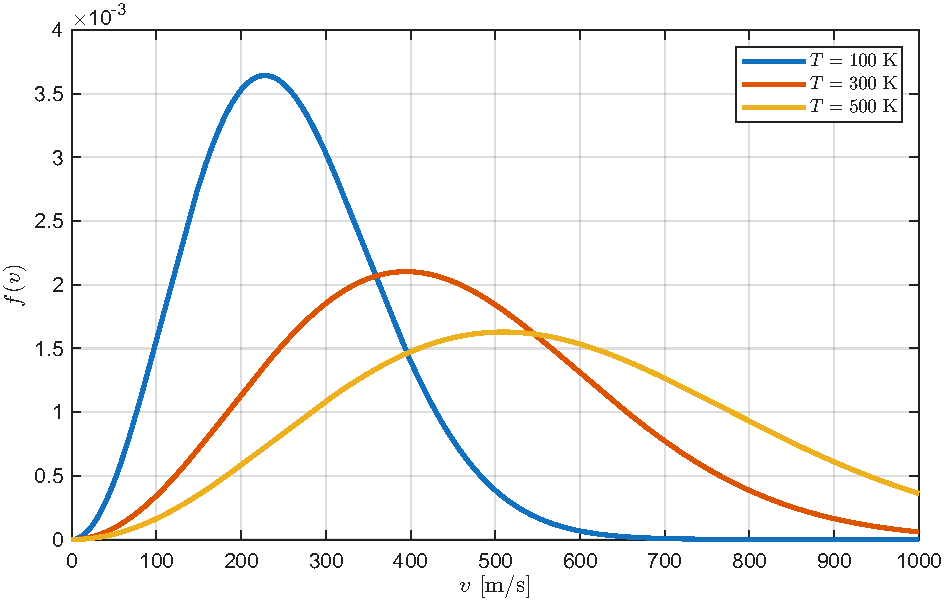
\includegraphics[width=0.8\linewidth]{figures/Maxwell_distribution.pdf}
		\captionof{figure}{氧气分子$\mathrm{O_2}$的Maxwell速度分布}
		\label{fig:Maxwell distribution}
	\end{center}
\end{theorem}

\begin{proof}
	动量在$\d p=\d p_x\nd p_y\nd p_z$范围内的粒子数密度为
	\[
		\e{-\alpha-\beta\varepsilon}\frac{\d p}{h^3}=\frac n{(2\pi m\kB T)^{3/2}}\e{-\beta(p_x^2+p_y^2+p_z^2)/2m}\d p_x\nd p_y\nd p_z,
	\]
	由$p_i=mv_i$,可得
	\begin{equation}
		f(v_x,v_y,v_z)\d v_x\nd v_y\nd v_z=n\biggkh{\frac m{2\pi\kB T}}^{3/2}\e{-m(v_x^2+v_y^2+v_z^2)/2\kB T}\d v_x\nd v_y\nd v_z.
	\end{equation}
	易证,$f(v_x,v_y,v_z)$是归一化的:
	\[
		\int\iti\int\iti\int\iti f(v_x,v_y,v_z)\d v_x\nd v_y\nd v_z=n.
	\]
	将坐标$(v_x,v_y,v_z)$换为球坐标$(v,\theta,\phi)$,并对$\theta,\phi$直接积分,便得到速率的分布。
\end{proof}

\begin{corollary}
	最概然速率$v_\mathrm m$、平均速率$\avg v$和方均根速率$v_\mathrm s$为
	\begin{subequations}
		\begin{align}
			v_\mathrm m&=\sqrt{\frac{2\kB T}m},\\
			\avg v&=\sqrt{\frac{8\kB T}{\pi m}},\\
			v_\mathrm s&=\sqrt{\frac{3\kB T}m}.
		\end{align}
	\end{subequations}
	单位时间碰撞单位面积器壁上的粒子数
	\begin{equation}
		\Gamma=\int\iti\int\iti\int\zti f(v_x,v_y,x_z) v_x\d v_x\nd v_y\nd v_z=\frac14n\avg v.
	\end{equation}
\end{corollary}

\subsection{振动}
\label{ssec:vibration}

考虑一维振动,%取约化质量$\mu$,
有
\[
	\varepsilon_\vb=h\nu\biggkh{n+\frac12},\quad\omega_\vb=1.
\]
能量间距$\D\varepsilon_\vb=h\nu\sim\SI{0.1}\electronvolt>\SI{0.025}\electronvolt$常温,因此必须考虑能级的分立性。
定义振动的特征温度
\[
	\theta_\vb:=\frac{\D\varepsilon_\vb}\kB=\frac{h\nu}\kB\sim\SI{e3}\K.
\]
则配分函数
\begin{equation}
	Z_\vb=\sum_n\omega_\vb\e{-\beta\varepsilon_\vb}=\sum_{n=0}^\infty\e{-(n+1/2)\beta h\nu}=\frac{\e{-\beta h\nu/2}}{1-\e{-\beta h\nu}}.
\end{equation}
内能和比热
\begin{subequations}
	\begin{align}
		U_\vb&=-N\pv{\ln Z_\vb}\beta=Nh\nu\biggkh{\frac12+\frac1{\e{\beta h\nu}-1}},\\
		C_{V,\vb}&=\pu[V]{U_\vb}T=N\kB\Einst\biggkh{\frac{\theta_\vb}T}.
	\end{align}
\end{subequations}
其中Einstein函数
\[
	\Einst(x):=\frac{x^2\e x}{(\e x-1)^2}=
	\begin{cases}
		1-\frac{x^2}{12}+\bigo(x^4),&x\ll 1,\\
		x^2\e{-x}+\bigo(x^2\e{-2x}),&x\gg 1.
	\end{cases}
\]
分别对应高温和低温极限。高温极限下,能量准连续,$U_\vb=N\kB T$,比热$C_{V,\vb}=N\kB$;而在低温极限下,比热
\begin{equation}
	C_{V,\vb}\simeq N\kB\biggkh{\frac{\theta_\vb}T}^2\e{-\theta_\vb/T},\quad T\ll\theta_\vb.
\end{equation}

\begin{center}
	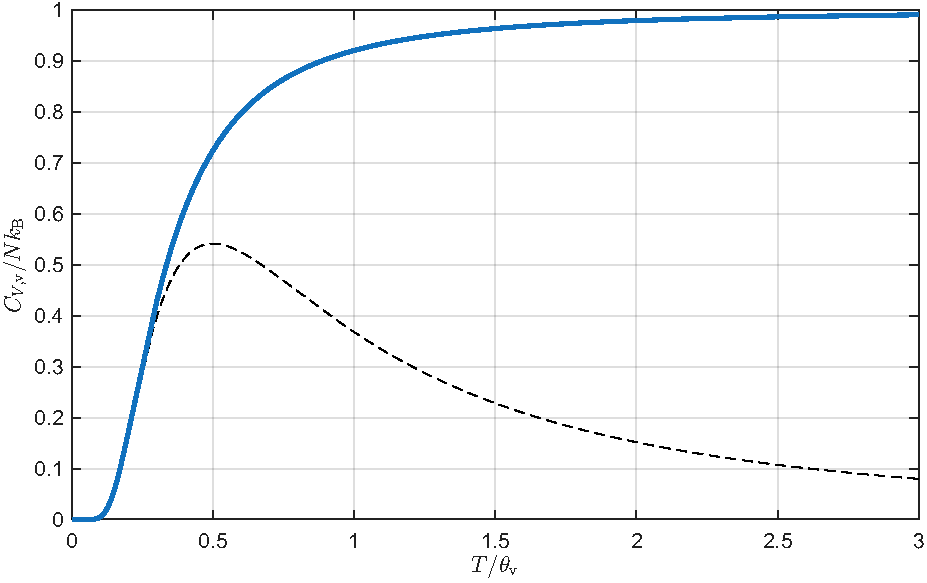
\includegraphics[width=0.8\linewidth]{figures/C_Vvib.pdf}
	\captionof{figure}{振动贡献热容$C_{V,\vb}\vs T$随温度的变化}
	\label{fig:C_Vvib - T}
\end{center}

\begin{example}
	{Einstein固体热容模型}{Einstein solid heat capacity model}

	讨论固体晶格振动对$C_V$的贡献。
	晶格间强耦合,当$T$不太高时,振幅小,晶格振动可约化为$3N$个独立、可区别的简谐振动。
	Einstein假设振动频率$\nu_i=\nu$是一样的,
	\[
		\varepsilon_n=h\nu\biggkh{n+\frac12},\quad n=0,1,2,\ldots
	\]
	和前面理想气体的振动类似,可得热容
	\[
		C_V=3N\kB\Einst\biggkh{\frac{\theta_{\Einst}}T},
	\]
	其中Einstein温度$\theta_{\Einst}=h\nu/\kB\sim\SIrange{100}{300}\K$。
	在低温下$C_V\propto T^{-2}\e{-\theta_{\Einst}/T}$与实验定性相符,定量不符。
	因为有低频模式在低温时仍能被激发,从而对$C_V$有贡献。(见Debye模型)

\end{example}

比较有三个自由度$p_x,p_y,p_z$的平动能量$U_\tl=3N\kB T/2$和有两个自由度的振动能量$U_\vb=N\kB T$,可以总结这样一个规律:

\begin{theorem}{能量均分定理}{energy equipartition}
	高温下,能量准连续,能量的每个自由度对能量贡献为$N\kB T/2$。
\end{theorem}

\begin{remark}
	原子内部结构(电子、原子核等)的自由度对宏观量(特别是$C_V$)无贡献。因为在稳定性、结合能、能级间距上,从分子、原子到原子核越来越稳定,特征温度越来越高,越来越难以被激发。即,结合的紧密的自由能被冻结了,通常不激发。
\end{remark}

\subsection{转动}
\label{ssec:rotation}

以异核双原子分子\footnote{同核需考虑全同性原理。比如正氢(两个氢核自旋平行) $\ell$为奇数;仲氢(两个氢核自旋反平行) $\ell$为偶数。}为例,
\[
	\varepsilon_\rt=\frac{\hbar^2}{2I}\ell(\ell+1),\quad\omega_\rt=2\ell+1.
\]
转动特征温度
\[
	\theta_\rt=\frac{\hbar^2}{2I\kB}\sim\SI{10}\K.
\]
高温下,能量准连续,可得内能$U_\rt=N\kB T$,比热$C_{V,\rt}=N\kB$符合能量均分定理;
低温下,配分函数并没有显式表达式,
\[
	Z_\rt=\sum_{\ell=0}^\infty(2\ell+1)\e{-\ell(\ell+1)\theta_\rt/T}=1+3\e{-2\theta_\rt/T}+5\e{-6\theta_\rt/T}+\bigo(\e{-12\theta_\rt/T}).
\]
只考虑$\ell=0,1$两项,可得
\begin{subequations}
	\begin{align}
		U_\rt&\simeq 6N\kB\theta_\rt\e{-2\theta_\rt/T},\\
		C_{V,\rt}&\simeq 12N\kB\biggkh{\frac{\theta_\rt}T}^2\e{-2\theta_\rt/T}.
	\end{align}
\end{subequations}
如图\figref{fig:C_Vrot - T} 所示,$C_{V,\rt}$并不是单调的,而是会有一个bump。

\begin{center}
	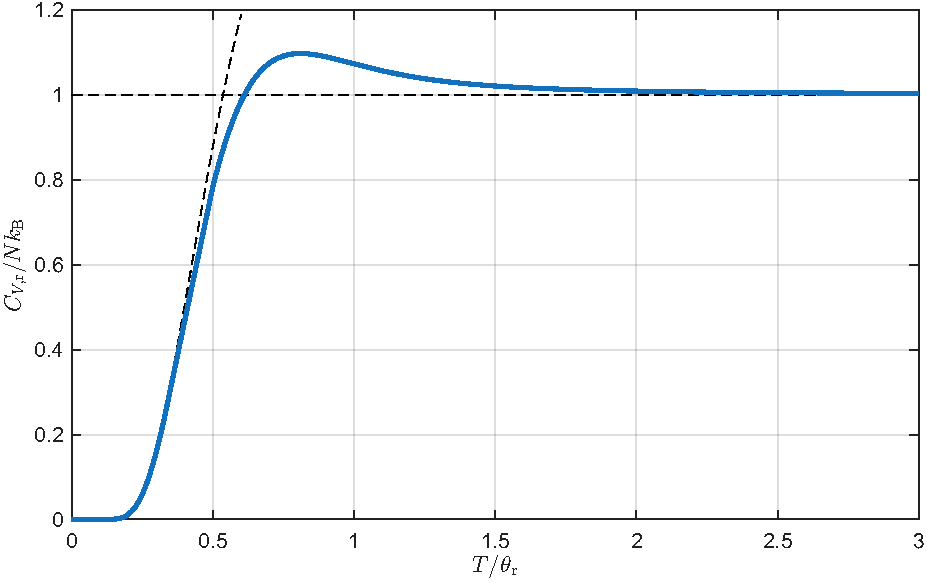
\includegraphics[width=0.8\linewidth]{figures/C_Vrot.pdf}
	\captionof{figure}{转动贡献热容$C_{V,\rt}\vs T$随温度的变化}
	\label{fig:C_Vrot - T}
\end{center}

总的内能和热容就是三种独立运动的和:
\[
	C_V=C_{V,\tl}+C_{V,\rt}+C_{V,\vb}.
\]
代入氧气$\mathrm{O_2}$的数据:$\theta_\rt=\SI{2.40}{K},\,\theta_\vb=\SI{2230}{K}$,可得理想气体模型下$\mathrm{O_2}$的总比热$C_V$随温度的变化如\figref{fig:C_V - T} 所示。
可见比热在相当长的一段温度范围内都是常数,当温度达到特征温度的量级后,对应部分的比热会开始出现,并在高温下符合能量均分定理。

\begin{center}
	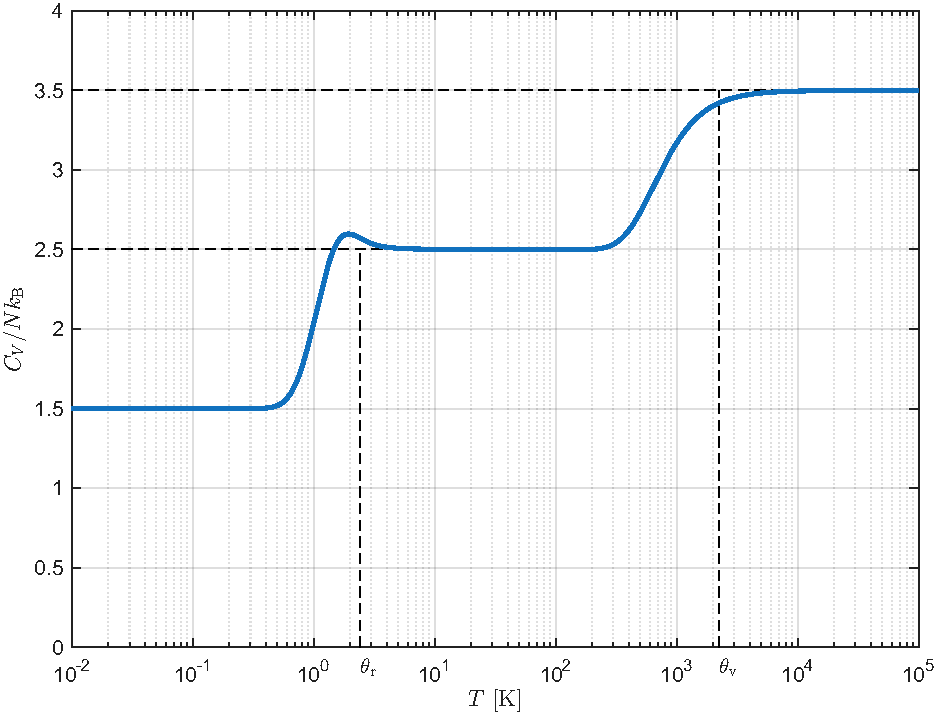
\includegraphics[width=0.8\linewidth]{figures/C_Vtot.pdf}
	\captionof{figure}{总热容$C_V\vs T$随温度的变化}
	\label{fig:C_V - T}
\end{center}

\section{顺磁性物质}

由量子力学,顺磁物质的粒子磁矩$\bm\mu$与总角动量$\bm J=\bm L+\bm S$成正比:
\[
	\bm\mu=g\muB\bm J,
\]
其中$\muB:=e\hbar/2m_\elc$为Bohr磁子,$g$为\Lande 因子。
\[
	g=1+\frac{j(j+1)+s(s+1)-\ell(\ell+1)}{2j(j+1)}.
\]
在外磁场$\bm B=\mu_0\bm H$下,单个粒子的能量为
\[
	\varepsilon_m=-\bm\mu\cdot\bm B=-\mu_0\muB g\bm J\cdot\bm H=-\mu_0\muB gHm,
\]
其中$m=-j,-j+1,\ldots,j$是$\bm J$在$\bm H$方向上的投影。
配分函数
\begin{equation}
	Z=\sum_{m=-j}^j\e{-\beta\varepsilon_m}=\frac{\e{aj}-\e{-a(j+1)}}{1-\e{-a}}=\division{\sinh\biggfkh{\biggkh{j+\frac12}a}}{\sinh\frac a2}.
\end{equation}
其中$a:=\beta\mu_0\muB gH$。
磁化强度、内能
\begin{subequations}
	\begin{align}
		M&=\frac N\beta\pv{\ln Z}{\mu_0H}=N\muB gj\Brill_j(a),\\
		U&=-N\pv{\ln Z}\beta=-\mu_0HM=-N\mu_0\muB gjH\Brill_j(a),
	\end{align}
\end{subequations}
其中Brillouin函数
\[
	\Brill_j(a):=\frac1j\hkh{\biggkh{j+\frac12}\coth\biggfkh{\biggkh{j+\frac12}a}-\frac12\coth\frac a2}.
\]
\begin{center}
	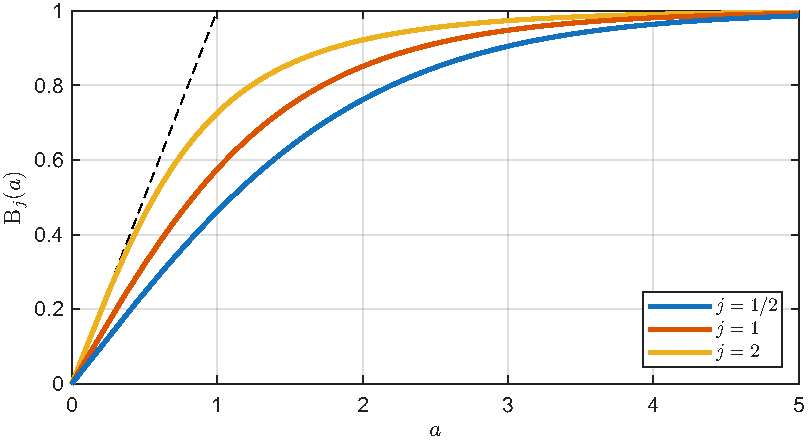
\includegraphics[width=0.8\linewidth]{figures/Brillouin.pdf}
	\captionof{figure}{Brillouin函数$\Brill_j(a)$}
	\label{fig:Brillouin function}
\end{center}

高温弱场极限下,$a\ll 1$,由$\coth$展开式可得
\[
	\Brill_j(a)=\frac{j+1}3a-\frac{(j+1)(2j^2+2j+1)}{90}a^3+\bigo(a^5).
	% \Brill_j(a)=\frac{j+1}3a-\frac{(j+1)[j^2+(j+1)^2]}{90}a^3+\frac{(j+1)[3j^2+(j+1)^2][j^2+3(j+1)^2]}{7560}a^5+\bigo(a^5).
\]
仅保留一阶项,
可得
\[
	M\simeq\frac{N\mu_0\muB^2g^2j(j+1)}{3\kB T}H,
\]
\begin{theorem}
	{Curie定律}{Curie's Law}
	顺磁物体的磁化强度$M=\chi H$与外场强度$H$成正比,且磁化率$\chi$与温度成反比:
	\begin{equation}
		\chi=\frac{N\mu_0\muB^2g^2j(j+1)}{3\kB T}\propto\frac1T.
	\end{equation}
\end{theorem}
低温强场极限下,$a\gg 1$,$\Brill_j(a)\simeq 1$
\[
	M\simeq N\muB gj.
\]
代表所有磁矩都与外场平行,达到饱和。

\paragraph{绝热退磁}

考虑Helmholtz自由能和熵
\begin{align*}
	F&=-\frac N\beta\ln Z=:\frac1\beta\phi(\beta H),\\
	S&=-\pv FT=\kB[-\phi(\beta H)+\beta H\phi'(\beta H)].
\end{align*}
绝热情况下,$S$不变,因此$\beta H=\const$。
即当外场$H$下降时,温度$T$也会下降,并且满足
\[
	T_\mathrm f=T_\mathrm i\frac{H_\mathrm f}{H_\mathrm i}.
\]
为实现这一效果,可选取$S(H=0)$随温度变化小的物质,比如$\mathrm{Ce_2Mg_3(NO_3)_{12}\cdot(H_2O)_{24}}$。

\section{负绝对温度}

1956年,Ramsey提出了有关负绝对温度的热力学与统计理论。根据
\[
	\frac1T=\pu[V,N]SU,
\]
一般情况下,内能越高,可能的微观状态数越多,熵越大,温度为正。但也有例外,这使负绝对温度的实现成为可能。

\paragraph{核自旋系统}

在外磁场$B$下,核自旋可以有两种取向,能量分别为$\pm\varepsilon$,
记两种取向的核磁矩数为$N_\pm$,
由系统的粒子数和能量关系:
\[
	\begin{cases}
		N=N_++N_- \\
		U=(N_+-N_-)\varepsilon
	\end{cases}
	\implies
	N_\pm=\frac N2\biggkh{1\pm\frac U{N\varepsilon}}.
\]
微观状态数$\Omega=N!/N_+!N_-!$,
熵
\begin{align*}
	S & =\kB\ln\biggkh{\frac{N!}{N_+!N_-!}}\simeq\kB(N\ln N-N_+\ln N_+-N_-\ln N_-).
	  \\& =N\kB\biggfkh{\ln 2-\frac12\biggkh{1+\frac U{N\varepsilon}}\ln\biggkh{1+\frac U{N\varepsilon}}-\frac12\biggkh{1-\frac U{N\varepsilon}}\ln\biggkh{1-\frac U{N\varepsilon}}}
\end{align*}
故温度的倒数
\begin{equation}
	\frac1T=\pu[V,N]SU=\frac\kB{2\varepsilon}\ln\biggkh{\frac{N\varepsilon-U}{N\varepsilon+U}}=\frac\kB{2\varepsilon}\ln\biggkh{\frac{N_-}{N_+}}
	\begin{cases}
		>0,&N_->N_+\\
		<0,&N_-<N_+
	\end{cases}
\end{equation}
当能量$U$从负转正的过程中,绝对温度的变化为
\[
	+T_0\enspace\longrightarrow\enspace+\infty\enspace\to\enspace -\infty\enspace\longrightarrow\enspace-T_0
\]
\begin{center}
	\includegraphics[page=22]{figures/tikz/coordinates.pdf}
	\captionof{figure}{$T\vs N_+$图像}
\end{center}

\begin{remark}
	实现负绝对温度的条件相当苛刻:
	\begin{compactenum}
		\item 系统的能量$U$有上界;
		\item 系统内部实现平衡(系统能与环境隔绝一段时间)。即
		\begin{center}
			系统本身达到平衡的弛予时间$\ll$系统与环境达到平衡的弛予时间
		\end{center}
		对于LiF晶体,前者为$\SI{e-5}\s$,后者为$\SI{5}\min$。
		1951年,Pursell和Pound在很纯的LiF晶体的核自旋系统中实现了负绝对温度的状态。
	\end{compactenum}
	只有满足以上条件,划分才有意义。
\end{remark}

